
\section*{Contemplación y EDGES} % Espacio para hablar del proyecto de (acomplete) de Dorian

\iffalse
\begin{itemize}
\item Distopía
\item domo 
\item Underborders
\item Milena y Concepción
\item setInterval()
\item Contemplación del fin del Mundo
\item sistemas mixtos
\item espacio y performance fusionados en Contemplación
\end{itemize}
\fi

\textit{Distopía}, \textit{NLXS + NK}, \textit{Interconexión}, \textit{setInterval()} y \textit{La Contemplación del Fin del Mundo} fueron los eventos realiados en el marco de \textit{EDGES}. 

\begin{figure}[H]
  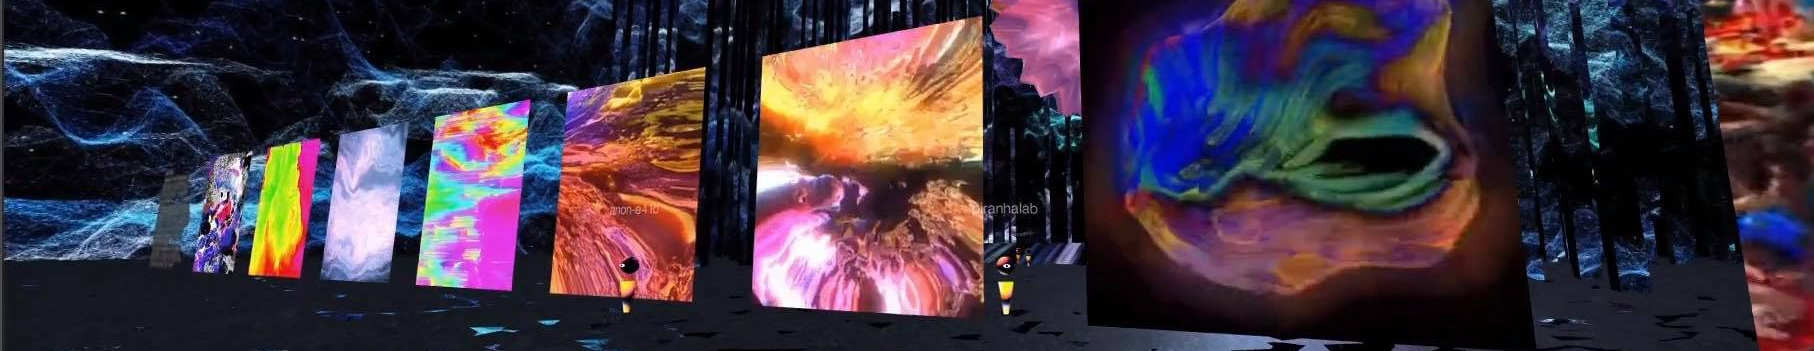
\includegraphics[width=\textwidth]{img/distopia.png}
  \caption{EDGES Distopía. Imágenes: LVSTVCRV}
\end{figure}

\textit{La Contemplación del Fin del Mundo} es un performance a modo de ejuego, último evento de la serie \textit{EDGES} que destruye el escenario de manera simbólica para dar por finalizado el ciclo de conciertos. Los asistentes podían presenciar el fin del mundo con la destrucción del escenario y otros eventos como inundaciones, objetos celestiales y finalmente la dispersión de los colores del escenario, dejando a los objetos del espacio sin razgos reconocibles.

La idea principal sirvió como vehículo para la exploración del espacio como característica del performance, el mundo explorable, la persecución en forma de figuras celestiales que ocupaban todo el espacio o que se expandían e iluminaban todo así como las inundaciociones. También permitió la exploración del uso de pantallas distribuidas a lo largo de todo el mundo, permitiendo a los usuarios presenciar el performance desde cualquier ubicación.

Uno de los aspectos a destacar de este concierto es el uso de acciones colectivas lanzadas por el artista, que durante el trascurso del evento podía cambiar las características del ambiente de manera similar entre los participantes. La experiencia de los usuarios fue se transformaba en el trancurso del evento, fue homogénea y compartida. Adicionalmente se implementó Hydra \citep{hydra} como un framework externo para la creación de visuales.

Las dificultad de las experiencias compartidas radica en la sincronización de eventos, tanto para los usuarios que ingresan desde el inicio o los usuarios ocasionales, sin importar ubicación geográfica o dispositivo. Esta posibilidad permite la interacción del artista y genera situaciones que añadan dinámica al juego, donde los asistentes se desplazan de ser observadores a ser participantes activos.

% Escribir sobre el proyecto de vincular threejs y hydra 
